\documentclass[a4paper,11pt,oneside]{book}

%%% το αρχείο αυτό καθορίζει το look που έχουν οι pythonies
%%% γίνεται \input από όλα τα κεφάλαια και τα φύλλα εργασίας

% χρησιμοποιούμενα πακέτα: 
% 
% polyglossia
% xstring
% graphicx
% caption
% xcolor
% hyperref
% minted
% geometry
% titlesec
% datetime
% changepage
% ntheorem

% οριζόμενες εντολές:
%
% smallcaps (βοηθ. removeaccents)
%    μικρά κεφαλαία χωρίς τόνους στα φωνήεντα
% scaling
%    η κλιμάκωση *όλων* των illustrations, τρέχουσα τιμή 0.9
% iconcomputer, iconkeyboard, icondiscuss, iconfillin, iconcaution, iconprompt, dottedline
%    εικονίδια για τα φύλλα εργασίας και εστιγμένη γραμμή
% marginnote
%    πλευρικό σχόλιο
% chapterwabstract (βοηθ. abstract, boxcolor, chaptercolor, concepts, tmpconcepts)
%    εισαγωγικό κείμενο κεφαλαίου με χρωματιστό τετράγωνο, συνοδευτικές έννοιες, κλπ.
% tobecontinued
%    εμφανίζει το "συνεχίζεται στην επόμενη σελίδα"

% οριζόμενα περιβάλλοντα:
% 
% note
%    μια υποσημείωση ή υπόδειξη, με μικρότερα γράμματα
% question
%    μια ερώτηση που "οδηγεί" κάθε νέα ενότητα
% answer
%    μια απάντηση σε μια ερώτηση του φύλλου εργασίας
% theory
%    μια ενότητα "θεωρίας" (στο τέλος ενός κεφαλαίου)
% exercise
%    μια αριθμημένη άσκηση
% step
%    ένα αριθμημένο βήμα (για φύλλο εργασίας)

% για μορφοποίηση κώδικα:
%
% pycode (περιβάλλον)
%     κώδικας python χωρίς αρίθμηση
% pyfile (εντολή)
%     εισαγωγή κώδικα python από αρχείο
% pyfilenl (εντολή)
%     εισαγωγή κώδικα python από αρχείο χωρίς αρίθμηση γραμμών
% pyfilesrc (εντολή)
%    εισαγωγή κώδικα από αρχείο με link στο αρχείο
% pyinline (εντολή)
%     κώδικας python μέσα στη ροή του κειμένου
% pyplain (περιβάλλον, για τα φύλλα εργασίας)
%     κώδικας python χωρίς φόντο
% pynew (περιβάλλον, για τα φύλλα εργασίας)
%     κώδικας python με φόντο
% pyterm (περιβάλλον για τα φύλλα εργασίας)
%     η είσοδος του χρήστη ή τα περιεχόμενα της οθόνης
% pyhighlight (εντολή)
%    highlight κειμένου (χρησιμοποιείται για κώδικα μέσα σε pyplain)


%%% επιλογές γλώσσας και γραμματοσειρών για το XeLaTeX

\usepackage{polyglossia}
\setdefaultlanguage{greek}
\setmainfont[Ligatures=TeX,SmallCapsFont={Linux Libertine O C},SmallCapsFeatures={Letters=SmallCaps}]{Linux Libertine O}
\setsansfont{Linux Biolinum O}
\setmonofont{Ubuntu Mono}
\enablehyphenation

% αφαίρεση τόνων από τα smallcaps
\usepackage{xstring}
\newcommand{\removeaccents}[1]{%
\def\result{#1}%
\StrSubstitute{\result}{ά}{α}[\result]%
\StrSubstitute{\result}{έ}{ε}[\result]%
\StrSubstitute{\result}{ή}{η}[\result]%
\StrSubstitute{\result}{ί}{ι}[\result]%
\StrSubstitute{\result}{ό}{ο}[\result]%
\StrSubstitute{\result}{ύ}{υ}[\result]%
\StrSubstitute{\result}{ώ}{ω}[\result]%
\StrSubstitute{\result}{Ά}{Α}[\result]%
\StrSubstitute{\result}{Έ}{Ε}[\result]%
\StrSubstitute{\result}{Ή}{Η}[\result]%
\StrSubstitute{\result}{Ί}{Ι}[\result]%
\StrSubstitute{\result}{Ό}{Ο}[\result]%
\StrSubstitute{\result}{Ύ}{Υ}[\result]%
\StrSubstitute{\result}{Ώ}{Ω}[\result]%
\result
}

\newcommand{\smallcaps}[1]{\textsc{\removeaccents{#1}}}

%%% εικόνες και λεζάντες

\usepackage{graphicx}
\newcommand{\scaling}{0.9}
\usepackage{caption}
\captionsetup{font=footnotesize}

%%% ειδικά περιβάλλοντα

\usepackage{xcolor}

% ερωτήσεις (που οδηγούν στην επόμενη ενότητα)
\definecolor{questioncolor}{rgb}{0.6,0.5,0.5}
\newenvironment{question}{\noindent\itshape\color{questioncolor}}{\noindent\ignorespaces}

% απαντήσεις (για τις ερωτήσεις των φύλλων εργασίας)
\definecolor{answercolor}{rgb}{0.5,0.5,0.5}
\newenvironment{answer}{\marginnote[16pt]{\iconfillin}\noindent\itshape\color{answercolor}}{\noindent\ignorespaces}

% περιβάλλον "θεωρίας" (πλήρες πλάτος κειμένου)
\usepackage{changepage}
\newenvironment{theory}[1]{\begin{adjustwidth}{}{-\overhang}\smallcaps{#1}\itshape}{\end{adjustwidth}}

% απομεινάρια...
% \newlength{\theoryrulelength}
% \setlength{\theoryrulelength}{36pt}
% \newenvironment{theory}{\rule{\theoryrulelength}{0.4pt}\begin{adjustwidth}{}{-\overhang}\itshape}{\end{adjustwidth}\rule{\theoryrulelength}{0.4pt}}

%%% υπερσύνδεσμοι

\definecolor{linkcolor}{rgb}{0.0,0.5,0.25}
\usepackage[colorlinks=true,urlcolor=linkcolor]{hyperref}

%%% εικονίδια και εστιγμένες γραμμές (για τα φύλλα εργασίας)

\newcommand{\iconcomputer}{
\includegraphics[scale=0.35]{../../share/circle-icons/one-color/computer.eps}}
\newcommand{\iconkeyboard}{
\includegraphics[scale=0.35]{../../share/circle-icons/one-color/keyboard.eps}}
\newcommand{\icondiscuss}{
\includegraphics[scale=0.35]{../../share/circle-icons/one-color/chat.eps}}
\newcommand{\iconfillin}{
\includegraphics[scale=0.35]{../../share/circle-icons/one-color/compose.eps}}
\newcommand{\iconcaution}{
\includegraphics[scale=0.35]{../../share/circle-icons/one-color/caution.eps}}
\newcommand{\iconprompt}{
\includegraphics[scale=0.35]{../../share/circle-icons/one-color/prompt.eps}}
\newcommand{\dottedline}{\vspace{\parskip}\dotfill}

%%% συνεχίζεται στην επόμενη σελίδα

\newcommand{\tobecontinued}{\mbox{}\hfill{\footnotesize ...συνεχίζεται στην επόμενη σελίδα.}}
\newenvironment{note}{\small\upshape}{}

%%% μορφοποίηση κώδικα με το pygmentize

\usepackage{minted}

% fix για ένα bug στο minted που εμφανίζεται όταν χρησιμοποιείται χρώμα στο φόντο (bgcolor)
% http://tex.stackexchange.com/questions/228058/how-to-space-before-and-after-a-minted-code-block-with-bgcolor
\makeatletter
\patchcmd{\minted@colorbg}{\noindent}{\noindent}{}{}
\apptocmd{\endminted@colorbg}{}{}{}
\makeatother

% χρώματα φόντου για τον κώδικα
\definecolor{codebg}{rgb}{0.80,0.95,0.85}
\definecolor{newcodebg}{rgb}{0.75,0.95,0.85}

% ορισμοί για τα περιβάλλοντα κώδικα
% pycode: περιβάλλον κώδικα python χωρίς αρίθμηση
\newminted[pycode]{python3}{bgcolor=codebg}
% pyfile: python από αρχείο
\newmintedfile[pyfile]{python3}{linenos=true,numberblanklines=false,escapeinside=||,bgcolor=codebg}
% pyfilenl: python από αρχείο χωρίς αρίθμηση γραμμών
\newmintedfile[pyfilenl]{python3}{linenos=false,numberblanklines=false,escapeinside=||,bgcolor=codebg}
% pyinline: python μέσα στη ροή του κειμένου
\newmintinline[pyinline]{python3}{linenos=true,numberblanklines=false}
% pyplain: (για τα φύλλα εργασίας) περιβάλλον χωρίς φόντο
\newminted[pyplain]{python3}{bgcolor=white,escapeinside=||,formatcom={\upshape}}
% pynew: (για τα φύλλα εργασίας) περιβάλλον με φόντο
\newminted[pynew]{python3}{bgcolor=newcodebg,escapeinside=||,formatcom={\upshape}}
% pyterm: (για τα φύλλα εργασίας) περιβάλλον για τα περιεχόμενα της οθόνης
\newminted[pyterm]{text}{bgcolor=white,escapeinside=||}

%\newminted[pyterm]{text}{escapeinside=||}
% [TODO] fix: το pyterm χωρίς bgcolor εμφανίζει μεγαλύτερα περιθώρια (πάνω και κάτω) και δεν φαίνεται ωραίο. Το bgcolor είναι προσωρινό workaround, έχει κι αυτό margins (για να μην είναι κολλητά ο κώδικας με το περιθώριο) κι έτσι ο κώδικας στ' αριστερά δεν είναι τέλεια στοιχισμένος.

% εντολή για κώδικα από αρχείο με link στο αρχείο
\newcommand{\pyfilesrc}[2][]{%
\pyfile[#1]{#2}\\
\mbox{}\hfill{\scriptsize\href{http://pythonies.mysch.gr/#2}{\url{#2}}}
}

% εντολή για το highlighting του κώδικα (συνήθως σε pyplain περιβάλλον με escapeinside)
\newcommand{\pyhighlight}[1]{\colorbox{newcodebg}{#1}}

%%% αριθμημένα περιβάλλοντα

\usepackage{ntheorem}

% άσκηση
\makeatletter
\theoremheaderfont{\upshape}%\upshape\bfseries\scshape}
\theorembodyfont{\itshape}%\slshape}
\newtheoremstyle{lmargin}%
  {\item[\theorem@headerfont \llap{##2}\hskip\labelsep\hskip-6pt]}%
  {\item[\theorem@headerfont \llap{##2}\hskip\labelsep ##1\ (##3)\theorem@separator]}
\makeatother
\theoremstyle{lmargin}
\newtheorem{exercise}{}[chapter]

% βήμα φύλλου εργασίας
\makeatletter
\theoremheaderfont{\bfseries}%\upshape\bfseries\scshape}
\theorembodyfont{\upshape}%\slshape}
\newtheoremstyle{lmarginup}%
  {\item[\theorem@headerfont \llap{##2}\hskip\labelsep\hskip-6pt]}%
  {\item[\theorem@headerfont \llap{##2}\hskip\labelsep ##1\ (##3)\theorem@separator]}
\newtheoremstyle{slmarginup}%
  {\item[\theorem@headerfont \llap{##1##2.}\hskip\labelsep\hskip-6pt]}%
  {\item[\theorem@headerfont \llap{##2.}\hskip\labelsep ##1\ (##3)\theorem@separator]}
\makeatother

% deprecated: \newcommand{\standalone}{} to define standalone
%\ifdefined\standalone
    \theoremstyle{slmarginup}
    \newtheorem{step}{}
%\else
%    \theoremstyle{lmarginup}
%    \newtheorem{step}{}[chapter]
%\fi

%%% γεωμετρία σελίδας και συναφείς ορισμοί από το tufte-latex
%%% https://tufte-latex.github.io/tufte-latex/

% εσοχή και διάστημα μεταξύ παραγράφων
% δεν επηρρεάζει το tufte-latex
\parindent=0pt
\parskip=6pt

% γεωμετρία σελίδας και ορισμός μηκών
\usepackage[a4paper,left=24.8mm,top=27.4mm,headsep=2\baselineskip,textwidth=107mm,marginparsep=8.2mm,marginparwidth=49.4mm,textheight=66\baselineskip,headheight=\baselineskip]{geometry}

\setlength{\marginparpush}{12pt}
\addtolength{\marginparpush}{\parskip}
\newlength{\fullwidth}
\setlength{\fullwidth}{\textwidth}
\addtolength{\fullwidth}{\marginparsep}
\addtolength{\fullwidth}{\marginparwidth}
\newlength{\overhang}
\setlength{\overhang}{\marginparsep}
\addtolength{\overhang}{\marginparwidth}

% απομεινάρια...
%\setlength\abovedisplayskip{6pt plus 2pt minus 4pt}
%\setlength\belowdisplayskip{6pt plus 2pt minus 4pt}

% italicize description run-in headings (instead of the default bold)
\renewcommand*\descriptionlabel[1]{\hspace\labelsep\normalfont\em #1}

% πλευρική σημείωση
\newcommand\marginnote[2][0pt]{%
  \marginpar{\hbox{}\vspace*{#1}\vspace*{-1\baselineskip}\noindent \footnotesize\textup{#2}}%
  {}%
}

% formatting title sections
\setcounter{secnumdepth}{-1}

\usepackage{titlesec}
\usepackage[nodate]{datetime}
\newlength{\beforesection}
\setlength{\beforesection}{3ex plus 0.5ex minus 0.2ex}
\addtolength{\beforesection}{-\parskip}
\newlength{\aftersection}
\setlength{\aftersection}{1.5ex plus 0.2ex}
\addtolength{\aftersection}{-\parskip}
\titlespacing*{\section}{0pt}{\beforesection}{\aftersection}

% απομεινάρια...
%\titlespacing*{\chapter}{0pt}{50pt}{40pt}
%\titlespacing*{\section}{0pt}{3.5ex plus 1ex minus .2ex}{2.3ex plus .2ex}

%%% για εισαγωγικό κείμενο κεφαλαίου με χρωματιστό τετράγωνο, συνοδευτικές έννοιες, κλπ.

\newcommand{\abstract}{}
\newcommand{\boxcolor}{}
\newcommand{\chaptercolor}{}
\newcommand{\concepts}{}
\newcommand{\tmpconcepts}{}
\newif\ifbonus

% reference: \titleformat{ command }[ shape ]{ format }{ label }{ sep }{ before-code }[ after-code ]
\titleformat{\chapter}[block]
{\Huge\sffamily}
{}
{0pt}
{\ifbonus\marginnote[-6pt]{\fcolorbox{\boxcolor}{\chaptercolor}{\makebox(40,40){\strut\textcolor{\boxcolor}{\Huge\thechapter}}}\\\vspace{\parskip}\\\tiny\today\\ \currenttime}\else\marginnote[-6pt]{\colorbox{\boxcolor}{\makebox(40,40){\strut\textcolor{\chaptercolor}{\Huge\thechapter}}}\\\vspace{\parskip}\\\tiny\today\\ \currenttime}\fi}
[\small\rmfamily\textmd\abstract\vspace{\parskip}\concepts\vspace{\parskip}\\\mbox{}\hrulefill]

\newcommand{\chapterwabstract}[5]{
	\renewcommand{\abstract}{#2}
    \renewcommand{\tmpconcepts}{#3}
	\ifdefempty{\tmpconcepts}{\renewcommand{\concepts}{}}{\renewcommand{\concepts}{\\\textbf{Έννοιες: }\tmpconcepts}}
	\renewcommand{\boxcolor}{#4}
	\renewcommand{\chaptercolor}{#5}
	\chapter{#1}
}

\definecolor{introColor}{rgb}{0.25,0.5,0.75}
\definecolor{answerColor}{rgb}{0.25,0.75,0.5}
\definecolor{crapsColor}{rgb}{0.5,0.75,0.25}
\definecolor{subtractionColor}{rgb}{0.5,0.25,0.75}
\definecolor{guessColor}{rgb}{0.75,0.25,0.5}
\definecolor{nimColor}{rgb}{0.75,0.5,0.25}
\definecolor{planetColor}{rgb}{0.25,0.25,0.75}
\definecolor{hangmanColor}{rgb}{0.25,0.75,0.25}
\definecolor{oxoColor}{rgb}{0.75,0.25,0.25}

\setcounter{part}{1}
\setcounter{chapter}{2}

%%% DOCUMENT START

\begin{document}

\chapterwabstract{Μπαρμπούτι}{Σε αυτό το κεφάλαιο θα φτιάξουμε ένα παιχνίδι με ζάρια. Στην πορεία θα εξασκηθούμε στη \emph{δομή επιλογής} και θα γνωρίσουμε τη \emph{δομή επανάληψης}, που μας επιτρέπει να εκτελούμε τις ίδιες εντολές πολλές φορές. Το τελικό πρόγραμμα θα είναι μικρό, όμως σύντομα θα χρειαστεί να γράψουμε προγράμματα μεγαλύτερα και πιο περίπλοκα. Έτσι, το ουσιαστικό αντικείμενο του κεφαλαίου είναι να έρθουμε σε επαφή με τον τρόπο που οι προγραμματιστές συνθέτουν τα προγράμματά τους από \emph{υποπρογράμματα}, σα να συναρμολογούν ένα περίπλοκο μηχάνημα από απλούστερα εξαρτήματα.}{δομή επιλογής, δομή επανάληψης, υποπρογράμματα}{crapsColor}{white}

Σε πολλές αμερικάνικες ταινίες οι πρωταγωνιστές κάνουν μια βόλτα από το Λας Βέγκας και γίνονται εκατομμυριούχοι ή χάνουν τα πάντα παίζοντας ένα παιχνίδι με ζάρια, άγνωστο στους περισσότερους. Η κοντινότερη ελληνική εκδοχή αυτού του παιχνιδιού είναι το μπαρμπούτι, πηγή έμπνευσης για πολλούς άτυχους ρεμπέτες.

Οι κανόνες είναι οι εξής: Αρχικά, ο παίκτης ρίχνει δύο ζάρια. Αν το άθροισμα των ενδείξεών τους είναι 4 ή 7, τότε ο παίκτης κερδίζει, ενώ αν είναι 2, 3 ή 11 χάνει. Σε οποιαδήποτε άλλη περίπτωση, το άθροισμα των ενδείξεων γίνεται ο ``στόχος'' και ο παίκτης ρίχνει \emph{επαναλαμβανόμενα} τα ζάρια μέχρι να ρίξει την ίδια ζαριά (να πετύχει τον στόχο), οπότε και κερδίζει, ή μέχρι να φέρει 7, οπότε και χάνει.

%%%%%%%%

\section{Τα Κόκκαλα Στον Μάστορα}

\begin{question}
Πώς θα προσομοιώσουμε το ρίξιμο των ζαριών;
\end{question}

Θα ασχοληθούμε αρχικά με την πρώτη ζαριά του παίκτη, με την οποία ξεκινά το παιχνίδι. Από την κατάλληλη \emph{βιβλιοθήκη} %
\marginnote[-6pt]{Για να χρησιμοποιήσουμε μια βιβλιοθήκη θα πρέπει πρώτα να την εισάγουμε (\pyinline{import}). Εδώ θα εισάγουμε τη βιβλιοθήκη \pyinline{random} και θα χρησιμοποιήσουμε την \pyinline{randint()}, που παράγει τυχαίους ακέραιους εντός καθορισμένων ορίων.}%
θα χρησιμοποιήσουμε έναν μηχανισμό παραγωγής τυχαίων αριθμών.

\marginnote{Εδώ η τιμή που επιστρέφει η \pyinline{input()}, δηλαδή το κείμενο που πληκτρολογεί ο χρήστης, δεν αποδίδεται σε κάποια μεταβλητή και χάνεται, αφού δεν μας ενδιαφέρει να τη διατηρήσουμε.}
\pyfile[firstline=1,lastline=7]{src/craps.1.py}

Ο παίκτης προτρέπεται να πατήσει το πλήκτρο \pyinline{ENTER} και, όταν το κάνει, οι μεταβλητές \pyinline{dice1} και \pyinline{dice2}, που αντιστοιχούν στις ενδείξεις των δύο ζαριών, παίρνουν μια τυχαία τιμή από το \pyinline{1} μέχρι και το \pyinline{6}. Μένει τώρα να εμφανίσουμε τη ζαριά στο χρήστη, αφού πρώτα υπολογίσουμε το άθροισμα των δύο ενδείξεων \pyinline{dice1} και \pyinline{dice2}.

\pyfile[firstline=8,lastline=10]{src/craps.1.py}

Η εντολή \pyinline{roll = dice1 + dice2} σημαίνει: υπολόγισε το άθροισμα των τιμών \pyinline{dice1} και \pyinline{dice2} κι ονόμασε το αποτέλεσμα \pyinline{roll}. Αυτό συμβαίνει \emph{μια φορά}, όταν εκτελείται η εντολή, και χρησιμοποιούνται οι τιμές που έχουν οι μεταβλητές \pyinline{dice1} και \pyinline{dice2} \emph{εκείνη την στιγμή}. 
%Αυτό \emph{δεν} σημαίνει ότι η μεταβλητή \pyinline{roll} θα είναι \emph{πάντα} ίση με το άθροισμα των δύο ζαριών, δηλαδή 
Αν οι \pyinline{dice1} και \pyinline{dice2} αλλάξουν τιμή, \emph{δεν} θα κάνει το ίδιο αυτόματα και η \pyinline{roll}. Η \pyinline{roll} θα αλλάξει τιμή μόνο όταν της αποδοθεί ρητά, με ένα \pyinline{=}, μια (οποιαδήποτε) άλλη τιμή.

%%%%%%%%

\section{Πάλι Ντόρτια Ήφερα}

\begin{question}
Και πώς θα ξέρουμε αν ο παίκτης κέρδισε, έχασε ή πρέπει να ξαναρίξει;
\end{question}

Στο σημείο αυτό %
\marginnote[2pt]{Κάθε \pyinline{if} συνοδεύεται από μια \emph{συνθήκη}, η οποία ελέγχεται κατά την εκτέλεση του προγράμματος και μπορεί να είναι αληθής (\pyinline{True}) ή ψευδής (\pyinline{False}).}%
\marginnote{Το \pyinline{elif} σημαίνει \pyinline{else if}. Μετά από μια \pyinline{if} μπορούμε να χρησιμοποιήσουμε όσες \pyinline{elif} είναι απαραίτητες.}%
\marginnote{Οι εντολές που ακολουθούν τις \pyinline{if} και \pyinline{elif} είναι στοιχισμένες δεξιότερα. Η στοίχιση υποδηλώνει ότι αυτές οι εντολές θα εκτελεστούν μόνο αν η αντίστοιχη συνθήκη είναι αληθής. Οι εντολές που ακολουθούν την \pyinline{else} είναι επίσης στοιχισμένες δεξιότερα και θα εκτελεστούν μόνο εφόσον οι προηγούμενες συνθήκες είναι ψευδείς.}%
\marginnote{Μην παραλείπετε το σύμβολο \pyinline{:} μετά τις συνθήκες και την \pyinline{else}.}%
\marginnote{Με το \pyinline{==} ελέγχεται αν δύο τιμές είναι ίσες. Διαφέρει από το \pyinline{=} που χρησιμοποιείται για να δώσουμε τιμή σε μια μεταβλητή.}%
\marginnote{Το \pyinline{or} χρησιμοποιείται για τη διάζευξη δύο συνθηκών. Η διάζευξη είναι αληθής όταν \emph{τουλάχιστον μια} από τις διαζευγμένες συνθήκες είναι αληθής. Υπάρχει και o τελεστής \pyinline{and}. Χρησιμοποιείται για τη \emph{σύζευξη} δύο συνθηκών, η οποία είναι αληθής όταν \emph{και οι δύο} συζευγμένες συνθήκες είναι αληθείς.}
υπάρχουν τρεις διαφορετικές περιπτώσεις, τρεις πιθανές εκδοχές για την συνέχεια του παιχνιδιού: νίκη (με 4 ή 7), ήττα (με 2, 3 ή 12) ή επανάληψη (σε οποιαδήποτε άλλη περίπτωση). Σε κάθε περίπτωση είναι διαφορετικές οι εντολές που θα πρέπει να εκτελεστούν, οπότε θα χρειαστούμε μια \emph{δομή επιλογής}, που θα μας επιτρέψει να \emph{ελέγξουμε} τη ζαριά του παίκτη, ώστε να εκτελέσουμε τις αντίστοιχες εντολές.

%Με άλλα λόγια, χρειαζόμαστε έναν τρόπο το πρόγραμμα να \emph{επιλέγει} την συμπεριφορά του ανάλογα με τις \emph{συνθήκες} που επικρατούν την ώρα της εκτέλεσής του.

\pyfile[firstline=11,lastline=21]{src/craps.1.py} 

Κατά την εκτέλεση του προγράμματος ελέγχονται διαδοχικά οι συνθήκες, η μία μετά την άλλη, μέχρι να βρεθεί μία που να είναι αληθής. Όταν συμβεί αυτό, εκτελούνται οι αντίστοιχες εντολές και δεν ελέγχεται καμία άλλη συνθήκη. Σε περίπτωση που διαπιστωθεί ότι όλες οι συνθήκες είναι ψευδείς, εκτελούνται οι εντολές της \pyinline{else}, αν υπάρχουν. Αυτό σημαίνει ότι τελικά θα εκτελεστούν \emph{μόνο} οι εντολές που αντιστοιχούν σε \emph{μία} από τις εναλλακτικές περιπτώσεις. 
%Τώρα που γράφουμε το πρόγραμμα, δεν είναι δυνατό να ξέρουμε εκ των προτέρων ποια θα είναι η ζαριά, οπότε πρέπει να καθορίσουμε τις εντολές που πρέπει να εκτελεστούν και στις τρεις πιθανές περιπτώσεις. Ωστόσο, 
%Κατά την εκτέλεση του προγράμματος, ανάλογα με τα αποτελέσματα που θα προκύψουν από τους ελέγχους των συνθηκών, θα εκτελεστούν \emph{μόνο} οι εντολές που αντιστοιχούν σε \emph{μια} από τις περιπτώσεις αυτές.

%%%%%%%%

\section{Ξανά Και Ξανά}

\begin{question}
Η τρίτη περίπτωση δεν είναι ολοκληρωμένη. Αν ο παίκτης δεν κερδίσει, ούτε χάσει με την πρώτη, πρέπει να ρίχνει συνεχώς ζαριές. Πώς θα κάνουμε τη διαδικασία αυτή να επαναλαμβάνεται;
\end{question}

Κάθε γλώσσα προγραμματισμού προσφέρει \emph{επαναληπτικές δομές}\marginnote{Στην Python, η βασική επαναληπτική δομή είναι η \pyinline{while}, η οποία μπορεί να χρησιμοποιηθεί σε κάθε περίπτωση, ενώ για συγκεκριμένου είδους επαναλήψεις υπάρχει και η δομή \pyinline{for}.}, δηλαδή τρόπους να εκφράσει κανείς ότι ένα σύνολο εντολών θα πρέπει να επαναλαμβάνεται.%
\marginnote{Η επαναληπτική δομή \pyinline{while} συνοδεύεται από μια \emph{συνθήκη συνέχειας}. Η συνθήκη ελέγχεται στην αρχή κάθε νέου κύκλου της επανάληψης και μπορεί να είναι αληθής (\pyinline{True}) ή ψευδής (\pyinline{False}). Όσο η συνθήκη είναι αληθής, η επανάληψη συνεχίζεται για άλλον έναν κύκλο.}
\marginnote{Μην παραλείπετε το σύμβολο \pyinline{:} μετά την συνθήκη.}%
\marginnote{Η τετριμμένη συνθήκη \pyinline{True} είναι πάντα αληθής κι έτσι η συγκεκριμένη επανάληψη δεν πρόκειται να διακοπεί λόγω της συνθήκης.} 
\marginnote{Οι εντολές που ακολουθούν τη \pyinline{while} είναι στοιχισμένες δεξιότερα. Η στοίχιση αυτή επιτυγχάνεται εισάγοντας κενά πριν από τις εντολές, τα οποία υποδηλώνουν ότι αυτές οι εντολές θα επαναλαμβάνονται. Η πρώτη εντολή μετά τη \pyinline{while} που δεν θα είναι στοιχισμένη δεξιότερα δεν θα επαναλαμβάνεται, αλλά θα εκτελεστεί μόνο μια φορά, όταν η επανάληψη τερματιστεί.}%
%Ο προγραμματιστής προσδιορίζει τις εντολές που εκτελούνται επαναλαμβανόμενα.%, αλλά και μια \emph{συνθήκη} που ελέγχεται σε κάθε κύκλο της επανάληψης και καθορίζει αν η επανάληψη πρέπει να συνεχιστεί ή όχι.
Μια τέτοια επαναληπτική δομή θα χρειαστεί να προσθέσουμε στην τρίτη περίπτωση, όπου ο παίκτης ούτε κερδίζει, ούτε χάνει με την πρώτη. Μέσα στην επανάληψη θα τοποθετήσουμε τις εντολές που υλοποιούν την ρίψη των ζαριών. Οι εντολές γράφονται μόνο μια φορά αλλά εκτελούνται ξανά και ξανά.

\pyfile[firstline=22,lastline=32]{src/craps.1.py}

%%%%%%%%

\section{Είναι Σημαντικό Να Έχεις Στόχους}

\begin{question}
Οι επαναλαμβανόμενες ρίψεις των ζαριών πρέπει κάποτε να σταματούν. Πώς τερματίζω την επαναληπτική διαδικασία;
\end{question}

%Οι εντολές που εμφωλεύτηκαν στην επαναληπτική δομή εκτελούνται \emph{συνεχώς} και ο παίκτης καλείται να ρίχνει ζαριές ακόμα κι όταν το παιχνίδι (θα πρέπει να) τελειώσει. 
Για να τερματίσουμε τον κύκλο της επανάληψης θα πρέπει μετά από κάθε ζαριά να \emph{ελέγξουμε} την έκβασή της. Υπάρχουν κι εδώ τρεις πιθανές περιπτώσεις: νίκη (ο παίκτης φέρνει ζαριά ίση με τον στόχο), ήττα (με 7) και συνέχεια της επανάληψης (σε οποιαδήποτε άλλη περίπτωση). Στις δύο πρώτες περιπτώσεις η επανάληψη θα πρέπει να τερματιστεί. Ένας απλός τρόπος για να επιτευχθεί αυτό είναι με την προσθήκη της εντολής \pyinline{break}, η οποία διακόπτει άμεσα τον κύκλο της επανάληψης.

\marginnote[18pt]{Η \pyinline{break} διακόπτει και τερματίζει \emph{άμεσα} τον κύκλο της επανάληψης, χωρίς να ελεγχθεί η συνθήκη συνέχειας.} 
\marginnote{Η \pyinline{else} δεν είναι υποχρεωτική σε μια δομή επιλογής και παραλείπεται όταν δεν υπάρχουν εντολές να εκτελεστούν στην τελευταία περίπτωση.} 
\pyfilesrc[firstline=33,lastline=41]{src/craps.1.py}
\clearpage

Η χρήση της \pyinline{break} είναι μια πρακτική που δεν ακολουθείται από όλους. Ορισμένοι θεωρούν ότι ο κώδικας είναι πιο κατανοητός όταν υπάρχει ένα μοναδικό σημείο εξόδου από την επανάληψη: η συνθήκη συνέχειας. Θα εξετάσουμε μια εκδοχή στην οποία ο κύκλος της επανάληψης δεν διακόπτεται άμεσα με την \pyinline{break} αλλά μόνο όταν η συνθήκη συνέχειας ελεγχθεί και διαπιστωθεί ότι είναι ψευδής.

%Είναι σημαντικό να συγκρίνετε το νέο αυτό πρόγραμμα με το προηγούμενο και να κατανοήσετε τον μηχανισμό τερματισμού της επανάληψης σε κάθε περίπτωση.

Θα χρησιμοποιήσουμε μια \emph{λογική} %
\marginnote[2pt]{Υπάρχουν μόνο δύο \emph{λογικές} τιμές: \pyinline{True} ή \pyinline{False}.}%, οι οποίες είναι τύπου \pyinline{bool}.}%
μεταβλητή \pyinline{over} για να ``θυμάται'' το πρόγραμμά μας αν το παιχνίδι έχει τελειώσει. Αρχικά, πριν την επανάληψη, η \pyinline{over} ορίζεται ως ψευδής (\pyinline{False}).

\pyfile[firstline=22,lastline=23]{src/craps.2.py}

Στην αρχή κάθε κύκλου της επανάληψης, ελέγχεται η συνθήκη συνέχειας \pyinline{not over}\marginnote{Το \pyinline{not} χρησιμοποιείται πριν από μια συνθήκη και \emph{αντιστρέφει} την τιμή της: όταν μια συνθήκη είναι ψευδής τότε η αντίστροφή της είναι αληθής και το ανάποδο.} κι ένας νέος κύκλος ξεκινά μόνο εφόσον η \pyinline{over} εξακολουθεί να είναι ψευδής.

\pyfile[firstline=24,lastline=25]{src/craps.2.py}

Η συνθήκη συνέχειας της επανάληψης θα μπορούσε εναλλακτικά να γραφτεί και με τους δύο ακόλουθους τρόπους:

\begin{pycode}
    # επανάληψη ρίψεων
    while over == False
\end{pycode}

\marginnote[28pt]{Με το \pyinline{!=} ελέγχεται αν δύο τιμές είναι διαφορετικές.}%
\begin{pycode}
    # επανάληψη ρίψεων
    while over != True
\end{pycode}

Η τιμή της \pyinline{over} θα πρέπει να αλλάζει σε αληθής (\pyinline{True}) όταν ο παίκτης κερδίσει ή χάσει -- εκεί δηλαδή όπου στην προηγούμενη εκδοχή συναντούσαμε την \pyinline{break}. 

\pyfilesrc[firstline=35,lastline=43]{src/craps.2.py}

Στην εκδοχή αυτή η επανάληψη \emph{δεν} θα σταματήσει άμεσα όταν η \pyinline{over} γίνει αληθής, αλλά όταν ελεγχθεί η συνθήκη συνέχειας και διαπιστωθεί ότι η \pyinline{over} είναι αληθής.

Μεταβλητές όπως η \pyinline{over} που παίρνουν μόνο δύο τιμές και χρησιμοποιούνται ως ένδειξη ότι κάποιο γεγονός έχει συμβεί ή όχι ονομάζονται συχνά \emph{σημαίες} (flags).
%\clearpage

%%%%%%%%

\section{Κάν'το Μου Λιανά}

\begin{question}
Το πρόγραμμα λειτουργεί, αλλά δεν μου αρέσει ο τρόπος που είναι γραμμένο. Οι εντολές για την ρίψη μιας ζαριάς επαναλαμβάνονται αυτούσιες σε δύο σημεία του προγράμματος. 
\end{question}

\marginnote[-50pt]{Tα υποπρογράμματα στην Python και σε πολλές άλλες γλώσσες έχουν τη μορφή \emph{συναρτήσεων}. Έχουν ένα όνομα και μια (προαιρετική) σειρά \emph{παραμέτρων}, εντός παρενθέσεων. Όταν κληθούν, οι συναρτήσεις δέχονται τιμές για τα ορίσματα, τα \emph{επεξεργάζονται} και \emph{επιστρέφουν} μια τιμή.}%
\marginnote{Έχουμε ήδη χρησιμοποιήσει συναρτήσεις που παρέχει έτοιμες η Python, όπως η \pyinline{print()} και η \pyinline{input()}, αλλά και συναρτήσεις που ανήκουν σε βιβλιοθήκες, όπως \pyinline{time.sleep()} και η \pyinline{random.randint()}. Τα προγράμματά μας καλούν αυτές τις συναρτήσεις κι αυτές εκτελούνται, παρέχοντας συγκεκριμένες λειτουργίες.}%
\marginnote{Εικόνα: Μια αναπαράσταση της συνάρτησης \pyinline{rollDice()}.\begin{center}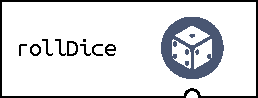
\includegraphics[scale=\scaling]{illustrations/rollDice.pdf}\end{center}}
\marginnote{Ο ορισμός μιας συνάρτησης ξεκινά με τη λέξη \pyinline{def} και ακολουθείται από το όνομα της συνάρτησης και τις παραμέτρους της, μέσα σε παρενθέσεις.}%
%\marginnote{Μην παραλείπετε το σύμβολο \pyinline{:} στο τέλος της πρώτης γραμμής.}%
\marginnote{Οι εντολές που ακολουθούν την πρώτη γραμμή είναι στοιχισμένες δεξιότερα. Η στοίχιση αυτή υποδηλώνει ότι οι εντολές αυτές θα εκτελεστούν όταν \emph{κληθεί} η συνάρτηση.}%
\marginnote{Το ειδικό σχόλιο στην αρχή της συνάρτησης, ανάμεσα στα 3 διπλά εισαγωγικά, χρησιμοποιείται για να περιγράψει τη λειτουργία της. Είναι προαιρετικό, όπως όλα τα σχόλια.}%
Οι ίδιες εντολές που προσομοιώνουν τη ρίψη των ζαριών χρησιμοποιούνται τόσο στην αρχική ζαριά όσο και στις επαναλαμβανόμενες ζαριές. 
Αυτές οι εντολές δεν είναι ούτε αναγκαίο, ούτε σκόπιμο να επαναλαμβάνονται. Ουσιαστικά, αποτελούν ένα ενιαίο σύνολο και υλοποιούν μια συγκεκριμένη λειτουργία. Μπορούμε λοιπόν να τις τοποθετήσουμε μέσα σ' ένα \emph{υποπρόγραμμα}, δημιουργώντας έτσι ένα κλειστό ``εξάρτημα'' που υλοποιεί την συγκεκριμένη λειτουργία της ρίψης των ζαριών.

\pyfile[firstline=2,lastline=15]{src/craps.3.py}

Το υποπρόγραμμα \pyinline{rollDice()} δεν δέχεται \emph{παραμέτρους} (γιατί δεν χρειάζεται εξωτερικές τιμές για να λειτουργήσει), και \emph{επιστρέφει} το άθροισμα των ενδείξεων των δύο ζαριών.

Προς το παρόν έχουμε μόνο \emph{ορίσει} το υποπρόγραμμα. Για να το χρησιμοποιήσουμε, ενεργοποιώντας την εκτέλεση των εντολών του, πρέπει να το \emph{καλέσουμε} στα δύο σημεία του προγράμματος όπου ο χρήστης ρίχνει τα ζάρια (αντί να παραθέτουμε τις αντίστοιχες εντολές).

\marginnote{Εικόνα: Η κλήση της \pyinline{rollDice()} από το κύριο πρόγραμμα. 
\begin{center}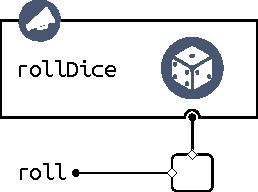
\includegraphics[scale=\scaling]{illustrations/rollDice-call.pdf}\end{center}
Αφού εκτελεστούν οι εντολές της, η συνάρτηση επιστρέφει μια τιμή. Εδώ η τιμή αυτή αποδίδεται στη μεταβλητή \pyinline{roll} του κύριου προγράμματος.}

\pyfile[firstline=16,lastline=17]{src/craps.3.py}

\pyfilesrc[firstline=33,lastline=34]{src/craps.3.py}

Σημειώστε ότι οι μεταβλητές \pyinline{dice1}, \pyinline{dice2} και \pyinline{roll} είναι \emph{τοπικές} στο υποπρόγραμμα. Δημιουργούνται κάθε φορά που αυτό καλείται και παύουν να υπάρχουν όταν ολοκληρωθεί η εκτέλεσή του. Στο κύριο πρόγραμμα υπάρχει επίσης μια (διαφορετική) μεταβλητή \pyinline{roll}, στην οποία αποδίδεται η τιμή που επιστρέφει η συνάρτηση \pyinline{rollDice()}.

%Μελετήστε το πλήρες πρόγραμμα στο τέλος του κεφαλαίου. Η χρήση του υποπρογράμματος το καθιστά πιο συμπαγές κι ευανάγνωστο, ενώ η δομή του ακολουθεί τη δομή των κανόνων του παιχνιδιού.

%%%%%%%%

\section{Πλήρες Πρόγραμμα}

\pyfilesrc{src/craps.final.py}

%%%%%%%%

\section{Ασκήσεις}

\begin{exercise}
Το «Ανάμεσα» ή «Acey Ducey» είναι ένα παιχνίδι με χαρτιά. Ο ένας παίκτης (η «μάνα») τραβάει δύο χαρτιά από την τράπουλα και τα δείχνει στο δεύτερο παίκτη. Εκείνος με την σειρά του στοιχηματίζει ένα ποσό και νικάει όταν το τρίτο χαρτί είναι ανάμεσα στα δύο πρώτα. Όσο πιο απίθανο είναι να νικήσει ένας παίκτης, τόσο μεγαλύτερο είναι το ποσό που θα κερδίσει. Συγκεκριμένα, αν υπάρχουν d χαρτιά ανάμεσα στα δύο πρώτα, τότε το ποσό που κερδίζει ο παίκτης σε περίπτωση νίκης θα είναι 12/d φορές το ποσό που στοιχημάτισε.

\begin{note}
Για παράδειγμα, αν τα δύο πρώτα χαρτιά είναι το 5 και το 8, τότε ο δεύτερος παίκτης θα νικήσει αν το επόμενο χαρτί είναι το 6 ή το 7 (d=2). Στην περίπτωση αυτή θα κερδίσει 6 φορές το ποσό που στοιχημάτισε.
\end{note}

Θεωρήστε ότι τα χαρτιά που χρησιμοποιούνται είναι από το 1 μέχρι και το 13 (τα τρία τελευταία αντιστοιχούν στον βαλέ, τη ντάμα και τον ρήγα). Αναπτύξτε πρόγραμμα το οποίο παράγει τυχαία τα δύο πρώτα χαρτιά της μάνας. Αυτά θα πρέπει να διαφέρουν αριθμητικά τουλάχιστον κατά δύο μονάδες, ώστε να υπάρχει περιθώριο για τουλάχιστον ένα χαρτί ανάμεσά τους (d\,$\geq$1), αλλιώς η μάνα θα πρέπει να μοιράσει δύο νέα χαρτιά. Στη συνέχεια, το πρόγραμμα ρωτά τον παίκτη το ποσό που επιθυμεί να στοιχηματίσει και παράγει το τρίτο χαρτί, εμφανίζοντας κατάλληλο μήνυμα με το ποσό που κέρδισε ή έχασε ο δεύτερος παίκτης.
\end{exercise}

\begin{exercise}
Να κατασκευάσετε ένα πρόγραμμα το οποίο θα παίζει το γνωστό παιχνίδι «Πέτρα-Ψαλίδι-Χαρτί» με το χρήστη. Σε κάθε γύρο, το πρόγραμμα θα ζητά από το χρήστη την επιλογή του (\textup{\pyinline{"Π"}}, \textup{\pyinline{"Ψ"}} ή \textup{\pyinline{"Χ"}}) και στη συνέχεια θα εμφανίζει τη δική του επιλογή και θα ανακοινώνει το νικητή του γύρου. Αν ο χρήστης πληκτρολογήσει οτιδήποτε εκτός από τις τρεις έγκυρες επιλογές τότε θεωρείται ότι επιθυμεί να τερματίσει το παιχνίδι. 

Μπορείτε να δοκιμάσετε και παραλλαγές του παιχνιδιού: τροποποιήστε το πρόγραμμα έτσι ώστε να επιλέγει από τις διαφορετικές κινήσεις με διαφορετική πιθανότητα ή κάντε το πρόγραμμα να κλέβει (μερικές φορές), επιλέγοντας κίνηση με βάση την κίνηση του χρήστη.
\end{exercise}

\begin{exercise} % Collatz
Το 1937, ο γερμανός μαθηματικός Lothar Collatz διατύπωσε τον παρακάτω ισχυρισμό, ο οποίος παραμένει αναπόδεικτος:
\begin{quote}
Επιλέξτε έναν θετικό ακέραιο n. Αν είναι άρτιος διαιρέστε τον με το 2, ενώ αν είναι περιττός πολλαπλασιάστε τον με το 3 και προσθέστε μια μονάδα. Επαναλάβετε τη διαδικασία με τον νέο αριθμό που θα προκύψει. Από οποιονδήποτε αριθμό n κι αν ξεκινήσετε, θα καταλήξετε στον αριθμό 1.
\end{quote}
Η εικασία %
\marginnote{\upshape\href{http://xkcd.com/710/}{\url{xkcd.com/710/}}}
έχει επαληθευτεί αριθμητικά μέχρι και για αριθμούς της τάξης των 6 δισεκατομμυρίων δισεκατομμυρίων, ωστόσο δεν υπάρχει αναλυτική μαθηματική απόδειξη. Θεωρητικά υπάρχει πάντα το ενδεχόμενο ένας ακόμα μεγαλύτερος αριθμός να παραβιάζει την εικασία!

\clearpage
Γράψτε ένα πρόγραμμα %
\marginnote{Για να διαπιστώσετε αν ένας αριθμός είναι περιττός ελέγξτε αν το υπόλοιπο της διαίρεσής του με το 2 είναι το 1.}%
το οποίο θα διαβάζει από το χρήστη τον αριθμό εκκίνησης n, θα επαναλαμβάνει τη διαδικασία 
που περιγράφεται παραπάνω και θα εμφανίζει τους διαδοχικούς αριθμούς που προκύπτουν από αυτή, έως ότου η διαδικασία καταλήξει στον αριθμό 1. Μπορείτε να εμπλουτίσετε το πρόγραμμά σας, ώστε μετά το τέλος της διαδικασίας να εμφανίζει το χρόνο τερματισμού, δηλαδή το συνολικό αριθμό των βημάτων που απαιτήθηκαν, αλλά και το σημείο πλημμυρίδας, δηλαδή τον μεγαλύτερο αριθμό που προέκυψε κατά την εκτέλεση της διαδικασίας.

\begin{note}
Για παράδειγμα, ξεκινώντας από το n=6 δημιουργείται η παρακάτω ακολουθία, με χρόνο τερματισμού τα 8 βήματα και σημείο πλημμυρίδας το 16:
\begin{center}
6\quad 3\quad 10\quad 5\quad 16\quad 8\quad 4\quad 2\quad 1
\end{center}
\end{note}

\end{exercise}

% άλλες ασκήσεις με ζάρια

%%%%%%%%

\section*{}
\vspace{-2\parskip}
\hrulefill

%\begin{theory}{Τελεστές και Εκφράσεις}
%\end{theory}

%\begin{theory}{Δομή Πολλαπλής Επιλογής}
%Πρόκειται για μια δομή \emph{πολλαπλής επιλογής}, αφού χρειάζεται να διακρίνουμε ανάμεσα σε περισσότερες από δύο περιπτώσεις.
%\end{theory}

\begin{theory}{Δομή Επανάληψης}
Η δομή επανάληψης μας δίνει τη δυνατότητα να περιγράφουμε διαδικασίες που επαναλαμβάνονται. Ίσως αρχικά αυτό να μην ακούγεται ιδιαίτερα εντυπωσιακό, γρήγορα όμως ανακαλύπτουμε ότι οι περισσότερες υπολογιστικές διαδικασίες είναι εγγενώς επαναληπτικές (αυτό περιλαμβάνει και τα περισσότερα \emph{παιχνίδια}) και είναι απαραίτητος ένας συμπαγής τρόπος περιγραφής τους. Με τη δομή επανάληψης περιγράφουμε τα βήματα ενός μόνο κύκλου, ακόμα κι αν τελικά αυτά τα βήματα θα εκτελεστούν πάρα πολλές φορές. 'Η ακόμα κι αν δεν γνωρίζουμε εκ των προτέρων πόσες φορές θα εκτελεστούν. Από μία άποψη, στις υπολογιστικές μας συσκευές ταιριάζει πολύ η δομή επανάληψης: σε αντίθεση με τους ανθρώπους, έχουν τη δυνατότητα να εκτελούν αδιαμαρτύρητα τα ίδια βήματα, ξανά και ξανά.
\end{theory}

\begin{theory}{Αναγνωσιμότητα και Break}
Σε μια επανάληψη μπορούμε να χρησιμοποιήσουμε μία ή και περισσότερες \pyinline{break}. Κάθε \pyinline{break} ανοίγει μια πόρτα εξόδου από τον κύκλο της επανάληψης. Επομένως, για να γνωρίζει κανείς πότε θα τερματιστεί μια επανάληψη θα πρέπει να αναζητήσει τις \pyinline{break} μέσα στην επανάληψη και να διαπιστώσει υπό ποιες συνθήκες θα εκτελεστούν. Αντίθετα, χωρίς την \pyinline{break}, η έξοδος από την επανάληψη γίνεται από ένα και μοναδικό σημείο: την συνθήκη συνέχειας. Η επανάληψη τερματίζεται μόνο όταν η συνθήκη συνέχειας ελεγχθεί και διαπιστωθεί ότι είναι ψευδής. Αρκεί λοιπόν να κοιτάξει κανείς την συνθήκη συνέχειας για να γνωρίζει πότε θα τερματιστεί μια επανάληψη. Φαίνεται λοιπόν ότι η άμεση διακοπή μιας επανάληψης με την \pyinline{break} είναι μεν συχνά βολική, όμως χωρίς την \pyinline{break} προκύπτουν προγράμματα που είναι περισσότερο κατανοητά και ευανάγνωστα. Αυτό είναι εξαιρετικά σημαντικό για κάποιους και πολύ λιγότερο για άλλους...
\end{theory}

\begin{theory}{Υποπρογράμματα}
Το μεγαλύτερο πλεονέκτημα που προκύπτει από τη χρήση υποπρογραμμάτων (και γίνεται πολύ εμφανέστερο καθώς τα προβλήματα και τα αντίστοιχα προγράμματα μεγαλώνουν) είναι ότι είμαστε ``αναγκασμένοι'' να αναλύουμε τα προβλήματα και να τ' αντιμετωπίζουμε \emph{τμηματικά}. Κάθε φορά εστιάζουμε την προσοχή μας σε μικρότερα κι απλούστερα κομμάτια του γενικού προβλήματος και στη συνέχεια, συνθέτουμε τη λύση, συναρμολογώντας τα κομμάτια αυτά. Στα κεφάλαια που ακολουθούν θα χρησιμοποιήσουμε περισσότερο τα υποπρογράμματα και θα αναφερθούμε εκτενέστερα στα πλεονεκτήματα που πηγάζουν από τη χρήση τους.

%Όπως οι λεπτομέρειες της λειτουργίας του υποπρογράμματος είναι κρυμμένες για εκείνους που απλά το χρησιμοποιούν, αντίστοιχα κρυμμένες είναι και τυχόν αλλαγές. Αν το υποπρόγραμμα τροποποιηθεί (επειδή βρήκαμε κάποιο λάθος, κάποιο τρόπο να λειτουργεί καλύτερα ή ακόμα και κάποια καλύτερη μέθοδο) οι αλλαγές θ' αφορούν μόνο το εσωτερικό του υποπρογράμματος, ενώ το υπόλοιπο πρόγραμμα θα παραμείνει αμετάβλητο.

%Ο τρόπος λειτουργίας της μεθόδου δεν είναι καθόλου προφανής. Αυτό όμως που μας ενδιαφέρει να δούμε εδώ είναι ότι η μέθοδος είναι ``κλεισμένη'' μέσα στην συνάρτηση. Όποιος θέλει να χρησιμοποιήσει την συνάρτηση δεν χρειάζεται να καταλαβαίνει πως λειτουργεί. Για την ακρίβεια, δεν χρειάζεται καν να γνωρίζει με ποια μέθοδο υπολογίζεται το αποτέλεσμα. Ο Al Sweigart, στο εξαιρετικό του βιβλίο Invent Your Own Computer Games with Python, γράφει: «Το ωραίο με τις συναρτήσεις είναι ότι χρειάζεται μόνο να ξέρουμε τι κάνουν, αλλά όχι πως το κάνουν.»

%Παράλληλα, το υποπρόγραμμα που αναπτύξαμε δεν λειτουργεί μόνο για έτη, μήνες και ημέρες, αλλά μπορεί να χρησιμοποιηθεί και σε οποιαδήποτε άλλη περίπτωση θέλουμε να διαβάσουμε από το χρήστη έναν ακέραιο αριθμό εντός ορίων. Με άλλα λόγια, το υποπρόγραμμα λύνει το πρόβλημα με γενικό τρόπο και είναι επαναχρησιμοποιήσιμο.

% ΣΧΟΛΙΟ: Παρακάτω θα εξετάσουμε κι άλλα πλεονεκτήματα των υποπρογραμμάτων
\end{theory}

\begin{theory}{Τυχαίοι Αριθμοί}
Η παραγωγή τυχαίων αριθμών έχει πολλές και σημαντικές εφαρμογές, όπως στην στατιστική, τις προσομοιώσεις και τα παιχνίδια, όμως η σημαντικότερη εφαρμογή της είναι στην \emph{κρυπτογραφία}. Υπάρχουν αρκετές υπολογιστικές μέθοδοι για να παράγει κανείς τυχαίους αριθμούς. Όλες τους ονομάζονται και \emph{γεννήτριες ψευδο-τυχαίων αριθμών} γιατί η αλήθεια είναι ότι οι αριθμοί που παράγουν \emph{φαίνονται} τυχαίοι, αλλά δεν είναι. Υπάρχουν μάλιστα και ειδικά στατιστικά κριτήρια που μετρούν πόσο απρόβλεπτες είναι οι ακολουθίες αριθμών που παράγονται. Η Python (και άλλες γλώσσες) χρησιμοποιoύν έναν αλγόριθμο που ονομάζεται Mersenne-Twister, ο οποίος είναι επαρκής για τις συνήθεις χρήσεις αλλά όχι για την κρυπτογραφία.
\end{theory}

\hrulefill

\end{document}

1.
% μήπως να το συγχωνεύαμε με το επόμενο;
A. Να υλοποιήσετε πρόγραμμα που θα προσομοιώνει τη ρίψη ενός νομίσματος και θα εμφανίζει μήνυμα «Κορώνα» ή «Γράμματα» αντίστοιχα.
B. Τροποποιήστε το παραπάνω πρόγραμμα, ώστε να το μετατρέψετε σε παιχνίδι. Αρχικά, το πρόγραμμα θα ζητά από τον παίκτη να επιλέξει Κορώνα ή Γράμματα, δίνοντας την αντίστοιχη λέξη. Το πρόγραμμα θα εμφανίζει στον παίκτη αν κέρδισε ή όχι, όπως παρακάτω.

2.
% εγκρίνεται, αλλά θέλει πολύ καλύτερη περιγραφή, δεν είναι ακριβώς έτσι τα πράγματα
% (αν το βάζαμε σε άλλο κεφάλαιο) μια συνάρτηση για ένα δίκαιο νόμισμα, μια για ένα biased και μια που να χρησιμοποιεί το biased για να φτιάχνει δίκαιο μαζί με προσομοιώσεις και ελέγχους
Ο αλγόριθμος του “δίκαιου” νομίσματος. Όταν ρίχνουμε ένα νόμισμα στο παιχνίδι “Κορώνα - Γράμματα” για να είμαστε σίγουροι ότι το νόμισμα είναι δίκαιο το ρίχνουμε 2 φορές. Αν και τις δύο φορές το νόμισμα πέσει από την ίδια πλευρά τότε η διαδικασία θεωρείται άκυρη και την επαναλαμβάνουμε. Αν οι 2 ρίψεις διαφέρουν τότε μετράει η αρχική ρίψη. Δηλαδή:
Κ → Γ	κερδίζει η Κορώνα
Γ → Κ κερδίζουν τα γράμματα
Γ → Γ ή Κ→ Κ η διαδικασία επαναλαμβάνεται
Να γραφεί πρόγραμμα που προσομοιώνει τον αλγόριθμο του δίκαιου νομίσματος.

7. 
% εγκρίνεται, με καλύτερη διατύπωση
11. Παιχνίδι μαθηματικών
% εγκρίνεται. αν είναι για παιδάκια, ίσως με κάποιους περιορισμούς (ο 2ος αριθμός να είναι μονοψήφιος).
Υλοποιήστε ένα πρόγραμμα που θα θέτει προβλήματα πρόσθεσης στον χρήστη του. Το πρόγραμμα θα παράγει δύο τυχαίους ακέραιους αριθμούς και θα ρωτά τον χρήστη ποιο είναι το αποτέλεσμα της πρόσθεσής του. Σε περίπτωση που ο χρήστης απαντήσει σωστά να εμφανίζει μήνυμα επιτυχίας διαφορετικά να του εμφανίζει τη σωστή απάντηση. 
Στη συνέχεια το πρόγραμμά σας θα ρωτά τον χρήστη αν θέλει να απαντήσει και σε άλλη ερώτηση και ανάλογα με την απάντησή του θα επαναλαμβάνει την παραπάνω διαδικασία. 
Σε κάθε επανάληψη να εμφανίζεται το πλήθος των σωστών και το πλήθος των λανθασμένων απαντήσεων.

